   
 
\documentclass[a4paper,10pt]{article}
\usepackage[utf8]{inputenc}
\usepackage[margin=25mm]{geometry}
\usepackage[italian]{babel}
\usepackage{amsmath}
\usepackage{amsthm}
\usepackage{amsfonts}
\usepackage{centernot}
\usepackage{multicol}
\usepackage{tikz}
\usepackage{listings}
\usepackage{courier}
\usepackage{MnSymbol}
\usetikzlibrary{patterns.meta}
\setlength{\parindent}{0em}
\newcommand{\reals}{\mathbb{R}}
\newcommand{\integers}{\mathbb{Z}}
\newcommand{\naturals}{\mathbb{N}}
\newcommand{\cnot}{\centernot}
\usepackage{graphicx}
\graphicspath{ {./images/} }

\definecolor{backcolour}{rgb}{0.95,0.95,0.92}
\lstdefinestyle{mystyle}{
    language=java,
    backgroundcolor=\color{backcolour},
    numberstyle=\tiny,
    basicstyle=\ttfamily\small,
    keywordstyle=\bfseries,
    breakatwhitespace=false,
    breaklines=true,
    captionpos=b,
    keepspaces=true,
    numbers=left,
    numbersep=5pt,
    showspaces=false,
    showstringspaces=false,
    showtabs=false,
    tabsize=2
}

\lstset{style=mystyle}

\begin{document}


\begin{center}
    \LARGE Giorno 6\smallskip

    \Large OOP: Generics in Java
\end{center}\smallskip

\begin{abstract}

\end{abstract}

\section{Generics}
[salto l'introduzione e le motivazioni (stesse di Typescript..), vd slide]
\subsection{Java Generics}
Prima dell'introduzione dei Generics in Java, l'unico modo per creare classi generiche era utilizzare il tipo Object e fare dei cast. Ora è tutto molto più efficiente:
\begin{lstlisting}
class Queue<T> {
    private T[] objects;
    ...
    public Queue(int size) {...}
    public boolean isFull() {...}
    public boolean isEmpty() {...}
    public void enqueue(T o) {...}
    public T dequeue() {...}
}

\end{lstlisting}

\subsection{Generics e nozione di sottotipo}
La nozione di sottotipo è \textbf{invariante} per le classi generiche, i.e. \[ Type2 \neq Type3 \quad\quad Type2 <: Type3 \quad\implies \quad Type1<Type2> \quad\not {<:} \quad Type1<Type3>\]

\paragraph{Nota:} in OCaml la nozione di sottotipo era \textbf{covariante}.

\paragraph{Esempi}
\begin{itemize}
 \item $Integer$ è sottotipo di $Number$
 \item $ArrayList<E>$ è sottotipo di $List<E>$ (poiché $ArrayList<E>$ implements $List<E>$)
 \item $List<E>$ è sottotipo di $Collection<E>$ (poiché $List<E>$ extends $Collection<E>$)
 \item \textbf{MA} $List<Integer>$ \textbf{NON è sottotipo} di $List<Number>$.
\end{itemize}
\subsubsection{Perché i generics di Java non sono covarianti?}
\label{dogcat}
Se Java ammettesse la covarianza sui tipi generici, si potrebbe avere:

\begin{lstlisting}
 List<Dog> dogs = new ArrayList<Dog>(); // ArrayList implements List
 List<Animal> animals = dogs; // Consentito se ammettesse covarianza
 animals.add(new Cat());
 Dog dog = dogs.get(0); // Qual e' il tipo effettivo di dog?
\end{lstlisting}

Non dobbiamo poter creare un alias con un tipo diverso! La stessa cosa potrebbe succedere con Integer e Number.\smallskip

Questo ci limita, nei casi in cui la nozione covariante non creerebbe problemi, ma almeno risolve un problema..

\paragraph{Perché in OCaml non c'è questo problema?} Perché le liste di OCaml non sono modificabili (quindi no alias).

\subsubsection{Limite superiore alla gerarchia}
Possiamo limitare un tipo generico:

\begin{lstlisting}
 interface List1<E extends Object> {...}
 interface List2<E extends Number> {...}
 List1<Date> // OK, Date e' un sottotipo di Object
 List2<Date> // compile-time error,
             // Date non e'
             // sottotipo di Number
\end{lstlisting}

Uso:

\begin{lstlisting}
 class List1<E extends Object> {
    void m(E arg) {
        arg.asInt();    // compiler error, E potrebbe
                        // non avere l'operazione asInt
        }
    }
    class List2<E extends Number> {
        void m(E arg) {
        arg.asInt();    // OK, Number e tutti i suoi
                        // sottotipi supportano asInt
    }
 } 
\end{lstlisting}

\subsubsection{Altri vincoli}

Abbiamo visto il vincolo \texttt{extends}: questo può anche essere multiplo:
\begin{lstlisting}
 <TypeVar extends ClassA & InterfB & InterfC & ... >
\end{lstlisting}

O si può avere un \textbf{limite inferiore}:
\begin{lstlisting}
 <TypeVar super SubType>
\end{lstlisting}
\subsection{Metodi generici}

\begin{itemize}
 \item I metodi possono usare le variabili di tipo dichiarate dalla classe
 \item I metodi possono anche dichiarare propri tipi generici: Segue ad esempio un metodo che copia liste di qualsiasi tipo
 \begin{lstlisting}
 <T> void copyTo(List<T> dst, List<T> src) {
    for (T t : src)
    dst.add(t);
 }
\end{lstlisting}

Anche meglio:
\begin{lstlisting}
<T1, T2 extends T1> void copyTo(List<T1> dst, List<T2> src) {
    for (T2 t : src)
        dst.add(t);
 }
\end{lstlisting}
Questo metodo è \textbf{più generico}, poiché può copiare gli elementi di una lista di tipo \texttt{List<T1>} in una lista di tipo \texttt{List<T2>}, a patto che \texttt{ T2 $<:$ T1}. 

\smallskip

Si noti che la variabile \texttt{T1} \textbf{non è utilizzata nel corpo}. \smallskip

\end{itemize}
\subsubsection{Wildcard}
In casi del genere, si può usare la \textbf{wildcard}: \texttt{?}

\begin{lstlisting}
 interface Set<E> {
    void addAll(Collection<? extends E> c);
    // Espressiva come: 
    <T extends E> void addAll(Collection<T> c);
}
\end{lstlisting}
\subsection{Array}
Gli array sono \textbf{covarianti}, scelta di implementazione fatta prima dei generics:

\[ Type1 <: Type2 \implies Type1[] <: Type2[] \]

Quindi: c'è ``il problema del cane e del gatto'' visto in \ref{dogcat}. 


\subsection{Type Erasure}
Divertentissimo: \textbf{tutti i tipi generici sono trasformati in Object} nel processo di compilazione, per backward-compatibiliy.\smallskip

Per questo motivo questo codice genera un warning:
\begin{lstlisting}
 List<?> lg = new ArrayList<String>( ); // ok
 List<String> ls = (List<String>) lg; // warning
\end{lstlisting}

Sto castando una lista di stringhe \textbf{nel suo stesso tipo}, ma il compilatore mi avverte che quel cast non sarà controllato a runtime, e sarà eseguito anche qualora fosse sbagliato.
\subsubsection{Sfruttare la type erasure per rompere Java}

\begin{lstlisting}
 import java.util.ArrayList;
 public class Prova<E extends Number> {
    public static void main(String[] args) {
        ArrayList<String> a = new ArrayList<String>();
        a.add("ciao");
        ArrayList<Integer> b = magic(a); // fa il cast...
        b.add(100);
        System.out.println(b.get(0)); // stampa "ciao"
        System.out.println(b.get(1)); // stampa 100
    }
        public static ArrayList<Integer> magic(ArrayList<?> a) {
        return (ArrayList<Integer>) a;
    }
 }
\end{lstlisting}

\newpage

\section{Java Collection Framework}
Una \textbf{collezione} è un insieme di oggetti \textbf{omogenei}, e.g. Liste, insiemi, code
\begin{center}
 
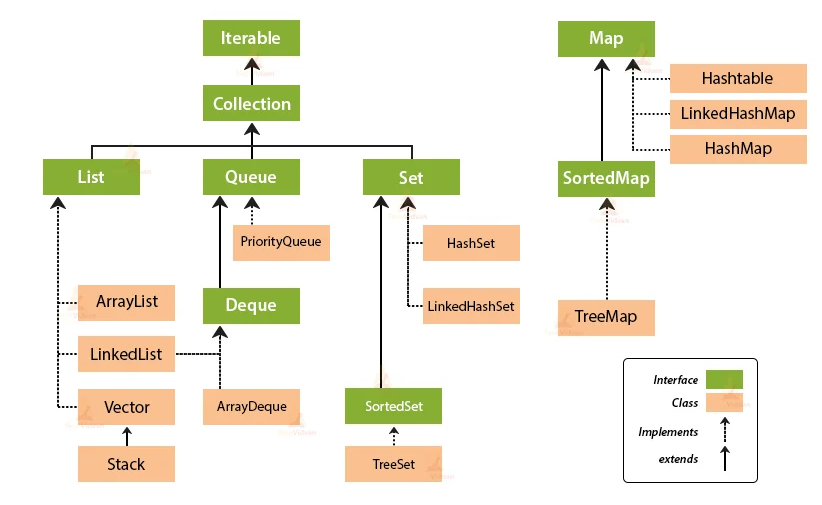
\includegraphics[scale = .5]{col}

\end{center}
\subsection{JCF in sintesi}
Il Java Collection Framework è un'architettura per rappresentare e manipolare collezioni; Consiste di una gerarchia di Abstract Data Type, con implementazioni ed algoritmi polimorfi (testati ed efficienti).\smallskip

\textbf{Collection$<E>$} è un'interfacciache definisce operazioni basiche su collezioni, e.g.:

\begin{itemize}
 \item \texttt{add (E e)}
 \item \texttt{remove (Object o)}
 \item \texttt{addAll(Collection<? extends E>)}
 \item \texttt{clear()}
  
\end{itemize}

Potremmo non volere implementare una o più di queste operazioni:
\begin{lstlisting} 
public boolean add(E e) {
    throw new UnsupportedOperationException( );
}
\end{lstlisting}
In questo modo possiamo definire una classe di collezioni \emph{non modificabili}.

Sono definiti anche degli ``observers'', tra cui: \texttt{contains(o), equals(o), isEmpty( ),
size( ), toArray()}.
\subsection{Principali interfacce}
\begin{itemize}
 \item $Set<E>$: collezione senza duplicati
 \item $List<E>$: sequenza lineare di elementi
 \item $Queue<E>$: Politica FIFO
 \item $Deque<E>$: ``double ended queue''
 \item $Map<K, T>$: \textbf{non estende Collection}; definisce associazione chiavi valori.
\end{itemize}\newpage
\subsection{Alcune classi:}
\begin{itemize}
 \item \texttt{ArrayList<E>}, \texttt{Vector<E>}: implementazione di \texttt{List<E>} basata su array
 \item \texttt{LinkedList<E>}: implementazione di list basata su lista doppiamente concatenata. Usa un record type Node.
 \item \texttt{TreeSet<E>} implementa set con ordine crescente degli elementi (ordine definito con \texttt{compareTo<E>})
 \item \texttt{HashSet<E>, LinkedHashSet<E>}: implementano set usando tabelle hash.
\end{itemize}
\subsection{Iterazione su collezioni}
Si noti che \texttt{Collection} non è la radice dell'albero: esiste un'\textbf{interfaccia Iterator} così definita:
\begin{lstlisting}
 public interface Iterator<E> {
    boolean hasNext( );
    E next( );
    void remove( );
 }
\end{lstlisting}
E così utilizzata:
\begin{lstlisting}
 // creo un iteratore sulla collezione
 Iterator<Integer> it = myIntCollection.iterator( );
 while (it.hasNext( )) {     // finche' ci sono elementi
    int x = it.next( );     // prendo il prossimo
    ...                     // uso x
 }
\end{lstlisting}

In particolare:
\begin{itemize}
 \item \texttt{hasNext()} restituisce \texttt{true} se l'iteratore ha altri elementi
 \item \texttt{next()} restituisce il prossimo elemento, o lancia un'eccezione se non ce ne sono
 \item \texttt{remove()} (operatore opzionale) rimuove dalla collezione l'ultimo elemento ritornato dall'iteratore.
\end{itemize}

\subsubsection{Iterazione, astraendo dalla collezione}

\begin{lstlisting}
 public static <E> void print(Collection<E> coll) {
    Iterator<E> it = coll.iterator();
    while (it.hasNext( )) // finche' ci sono elementi
    System.out.println(it.next( ));
 } 
\end{lstlisting}

\subsubsection{Il comando for-each (enhanced for)}
\begin{lstlisting}
 for (E elem : arr) System.out.println(elem);
\end{lstlisting}

\subsubsection{Uso degli iteratori}
Come esempio creiamo una classe iterabile \texttt{Primes}, con un iteratore che produce tutti i numeri primi una sola volta, in ordine crescente.

\begin{lstlisting}
 public class Primes implements Iterable<Integer> {
    public Iterator<Integer> iterator( );
        // EFFECTS: ritorna un iteratore che produrra' tutti i numeri
        // primi (come Integers) ciascuno una sola volta, in ordine
        //crescente
    }
    public static void printPrimes (int m) {
        // EFFECTS: stampa tutti i numeri primi minori o uguali a m
        // su System.out
        for (Integer p : new Primes( )){
            if (p > m) return; // forza la terminazione
            System.out.println("The next prime is: " + p);
        }
 }
\end{lstlisting}
La funzione \texttt{iterator} deve ritornare un iteratore con determinate caratteristiche. Dove lo definisco?
\newpage
\subsubsection{Implementazione degli operatori}
\textbf{Problema:} L'iteratore deve poter accedere alla rappresentazione interna della struttura dati, ma è una classe diversa! $\implies$ si scrive l'iteratore in una \textbf{classe annidata}.\smallskip

\textbf{Esempio:}
\begin{lstlisting}
 public class IntSet implements Iterable<Integer> {
    private int[] a;
    private int size;
    
    public IntSet(int capacity) { ... }
    public boolean add(int elem) throws FullSetException { ... }
    public boolean contains(int elem) { ... }
    
    public Iterator<Integer> iterator( ) {
        return new IntSetIterator();
    }
    // INNER CLASS (CLASSE INTERNA)
    private class IntSetIterator implements Iterator<Integer> {
        private int curr=0;
        public boolean hasNext() { return (curr<size); }
        public Integer next() {
        if (curr>=size) throw new NoSuchElementException();
            return a[curr++];
        }
        public void remove( ) {
            throw new UnsupportedOperationException( );
        }
    }
 }
\end{lstlisting}

Avrei anche potuto utilizzare una \textbf{classe anonima}:
\begin{lstlisting}
 public class IntSet implements Iterable<Integer> {
    ...
    public Iterator<Integer> iterator( ) {
        // INNER CLASS ANONIMA
        return new Iterator<Integer>() {
            private int curr=0;
            public boolean hasNext() { return (curr<size); }
            public Integer next() {
            if (curr>=size) throw new NoSuchElementException();
                return a[curr++];
            }
            public void remove( ) {
                throw new UnsupportedOperationException( );
            }
        };
    }
    
    
 }
\end{lstlisting}

\subsubsection{Interfaccia ListIterator}
Permette di spostarsi avanti ed indietro, e di aggiungere/settare elementi alla/della lista.

\subsubsection{Classi non modificabili}

La classe \textbf{Collections} (una classe che fornisce metodi di utilità per collezioni), forninsce un metodo \texttt{unmodifiableCollection} che prende una collezione e restituisce una versione non modificabile della stessa.

\end{document}
